



\begin{frame}\frametitle{LCRs - Low-Copy Repeats}  
\begin{itemize}
 \item also known as Segmental Duplications,
 \item DNA fragments $>$ 1 kb and $>$ 90\% DNA sequence identity
 \item LCRs $> 10$ kb and $>$ around $97\%$ sequence identity can lead to local genomic instability.
 \item may stimulate and/or mediate constitutional (both recurrent and nonrecurrent), evolutionary, and somatic genomic rearrangements
 \item may cause Non Allelic Homologous Recombination (NAHR) 
\end{itemize}
\end{frame}

% \section{LCRs, NAHR and genome rearrangements}
\begin{frame}\frametitle{LCRs, NAHR and genome rearrangements}  
	    \begin{center}
	   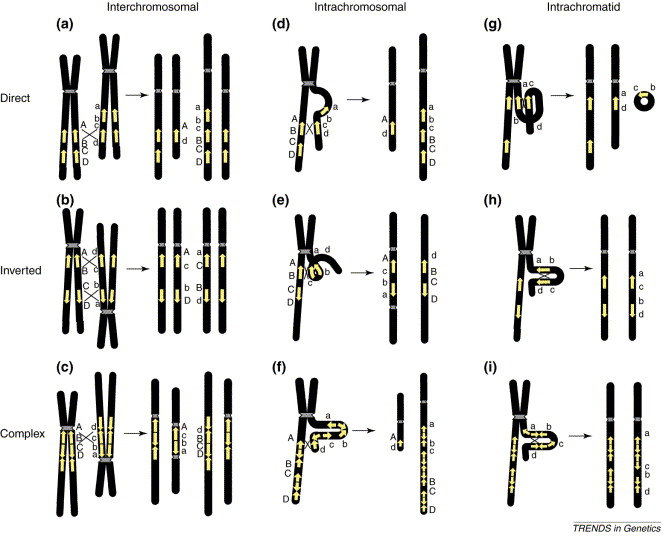
\includegraphics[width=0.9 \textwidth]{new-images/NAHR-LCRs.jpg}\\
	   \tiny{source: Stankiewicz et al., 2002}  
	    \end{center}
\end{frame}

% \section{IP-LCRs and inversion mechanism}
% \begin{frame}\frametitle{Inverted paralogous LCRs and inversion mechanism}
% 	    \begin{center}
% 	   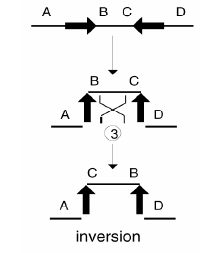
\includegraphics[width=0.5 \textwidth]{new-images/inversion.png}\\
% 	   \tiny{source: Gu et al., 2008}  
% 	    \end{center}
% \end{frame}

\begin{frame}\frametitle{Heamophilia A}

 \begin{columns}
    \column{0.35\textwidth}
	    \begin{center}
	   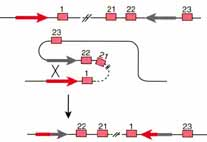
\includegraphics[width=0.95 \textwidth]{new-images/hemophiliaA.jpg}\\
	   \tiny{source: http://carolguze.com/text/442-2-mutations.shtml}  
	    \end{center}
    \column{0.65\textwidth}
\begin{itemize}
 \item recessive X-linked genetic disorder
 \item impair the body's ability to control blood clotting or coagulation %, which is used to stop bleeding when a blood vessel is broken
 \item present in about 1 in 5,000-10,000 male births
%  \item mutation in the Factor VIII (F8) gene (interupting the coding sequence and inactivating the gene)
\item single inversion disrupting the factor VIII gene (F8) accounts for $>$ 45\% of severe cases
 
\end{itemize}
\end{columns}
\end{frame}

\begin{frame}\frametitle{X-linked disorders}
	    \begin{center}
	   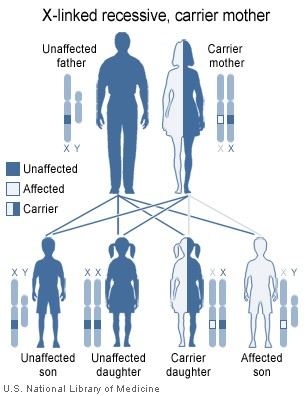
\includegraphics[width=0.5 \textwidth]{new-images/XlinkRecessive.jpg}\\
	   \tiny{X-linked recessive inheritance, source: wikipedia}  
	    \end{center}
\end{frame}



\begin{frame}\frametitle{Hunter syndrome (mucopolysaccharidosis Type II)}

 \begin{columns}   
    \column{0.65\textwidth}
\begin{itemize}
 \item recessive X-linked genetic disorder
 \item impair the body's ability to control blood clotting or coagulation %, which is used to stop bleeding when a blood vessel is broken
 \item affects approximately 1 in 155,000 live male births (rarely reported to occure also in females)%present in about 1 in 5,000-10,000 male births
 \item caused by a deficient (or absent) enzyme, iduronate-2-sulfatase (I2S)
 \item ~ 13\% of patients have the IDS gene disrupted by an NAHR-mediated inversion between the IDS gene and its pseudogene
 \end{itemize}

 \column{0.35\textwidth}
	    \begin{center}
	    
\includegraphics[width=0.95 \textwidth]{new-images/szymon-cajmer900w.jpg}\\
	    \tiny{http://davechidley.ca/news/}
	   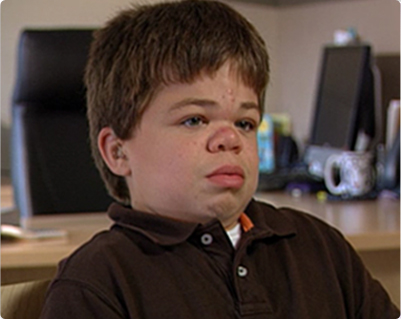
\includegraphics[width=0.95 \textwidth]{new-images/hero.jpg}\\
	    \tiny{http://www.hunterpatients.com/hunter-syndrome-community/}            
	    \end{center}



\end{columns}
\end{frame}



\begin{frame}\frametitle{Segmental Dups}  
\begin{itemize}  
 \item track at UCSC Genome Browser (http://genome.ucsc.edu)  
 \item Duplications of $>$ 1000 Bases of Non-RepeatMasked Sequence
\end{itemize}
\begin{center}
	   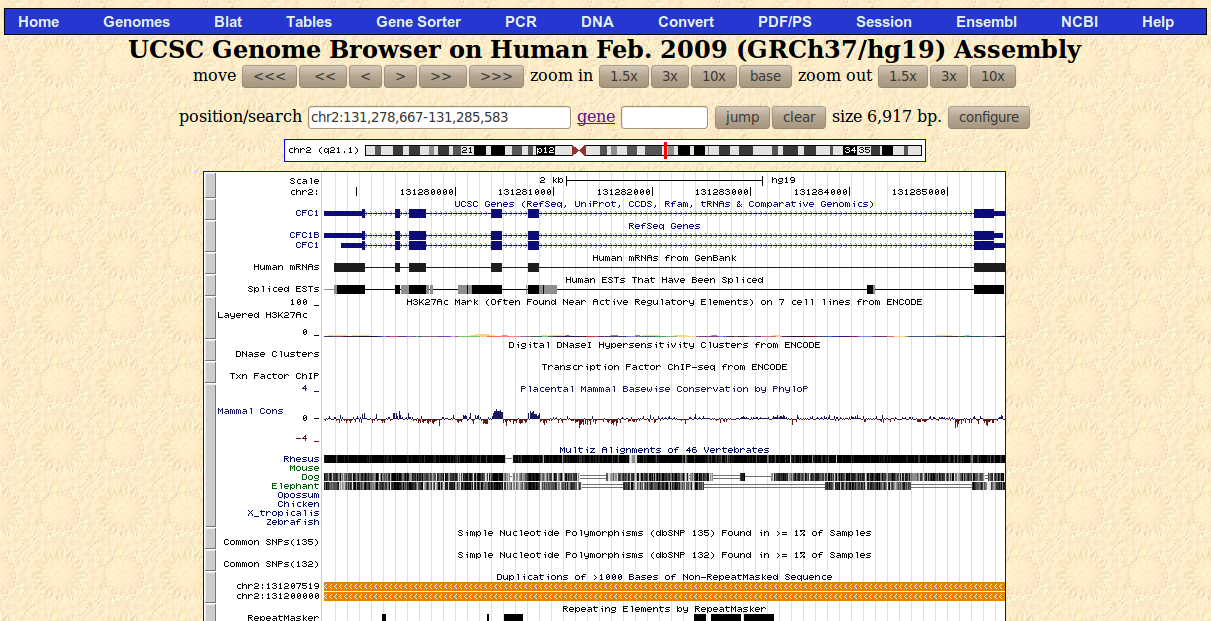
\includegraphics[width=0.9 \textwidth]{new-images/UCSC.png}\\	   
	    \end{center}
\end{frame}








\begin{frame}\frametitle{IP-LCRs}  
\begin{itemize}
 \item inversed paralogous LCRs (from SegDups)
 \item fraction matching (fractMatch) measure between paralogous elements at least 97\%, 
 \item distance between elements $<$ 10 Mb 
 \item minimal length of an element: 1 kb (limitation of SegDups track)
\end{itemize}
\end{frame}


\begin{frame}\frametitle{Pathogenic inversions}  
\begin{table}[t!]
\caption[Six pathologic inversions~ from~\cite{antonacci}]{Six pathologic inversions reported in~(Antonacci et al.). Last three columns corresponds to different LCR intersection requirements:
\textbf{strict}: intersection of inversion with 1Mbp region flanked by LCR pair, \textbf{mild}: intersection of inversion with 10Mbp region flanked by LCR pair, 
\textbf{intermediate}: intersection of inversion with any of LCR's separated by maximum 10 Mbp.
%\\\textbf{PD: Uwaga: ciekawe jest to, ze prawie wszystkie przeciecia z mild znajduja sie w intermediate. Ponadto jesli przetniemy choroby z LCR regions 1MB (strict) to 
%wynik jest taki sam, co gdybysmy przecieli je tylko z IP-LCRami}
}
\label{t:six}
\begin{center}
\begin{tabular}{c|c|c|c|c|c|c}
id & chrom & Start & End & strict & intermediate  &mild \\\hline
1 & chr3 & 195397784 & 197386290 & 1 & 2 & 2\\\hline
2 & chr8 & 7238551 & 12442658 & 6 & 9 & 9\\\hline
3 & chr15 & 30736914 & 32815174 & 5 & 13 & 14\\\hline
4 & chr15 & 74364359 & 75569130  & 0 & 2 & 2\\\hline
5 & chr17 & 34814327 & 36297053 & 1 & 5 & 5\\\hline
6 & chr17 & 43544137 & 44633937  & 5 & 7 & 8\\
\end{tabular}
\end{center}
\end{table}
\end{frame}



\begin{frame}\frametitle{Database of Genomic Variants (DGV)}  
\begin{itemize} 
 \item Structural Variations track in the UCSC browser, 
 \item healthy samples,
 \item DGV contains many false positives (e. g. small aberrations detected by poor–resolution technology have overestimated boundaries), so we filter out aberrations smaller than 10 Kbp,
 \item 925 inversions included in DGV, among them:
  \begin{itemize}
  \item 361 captured by DNA sequencing 
  \item 556 captured by Paired End Mapping (PEM)
  \end{itemize}
\end{itemize}
\end{frame}


\begin{frame}\frametitle{Inversions from DGV} 

%  \begin{columns}
%    \column{0.5\textwidth}
 
 	    \begin{center}
	   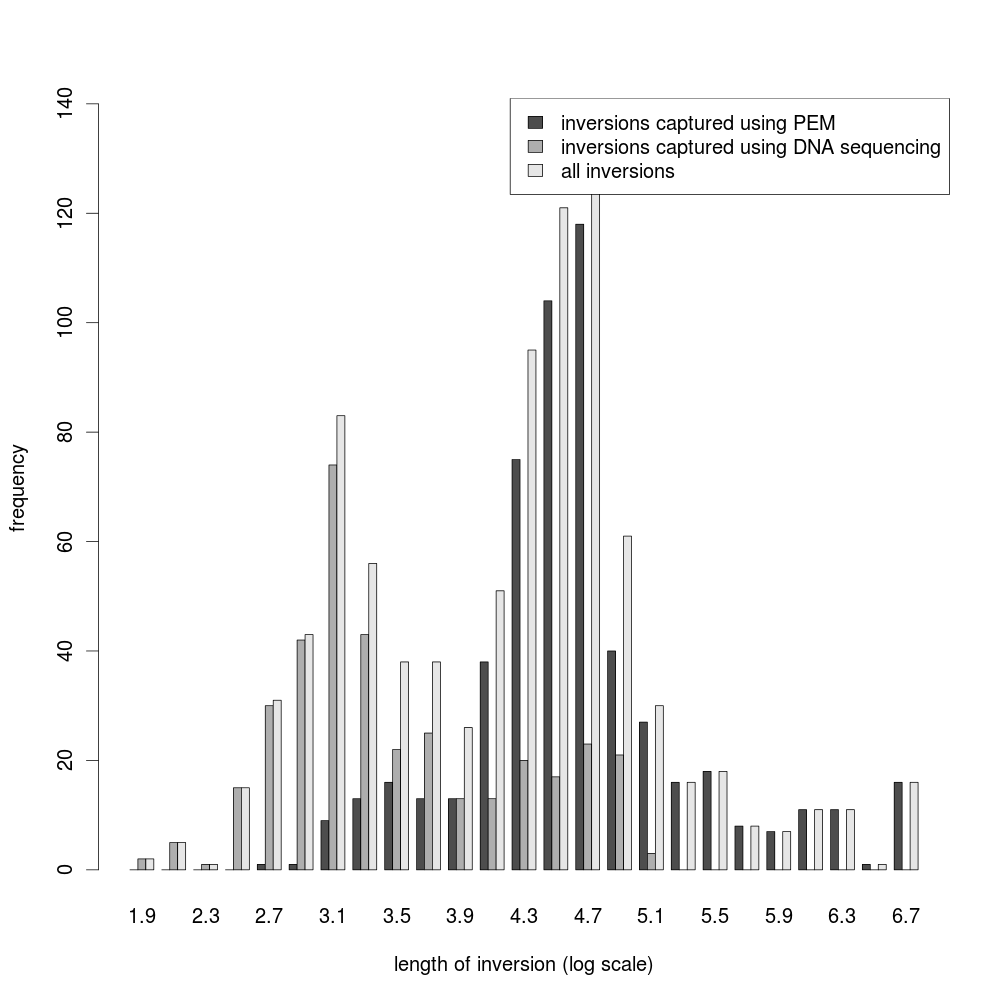
\includegraphics[width= 0.65\textwidth]{new-images/hist_inv_length.png}\\
% 	   \tiny{source: Stankiewicz et al., 2002}  
 	    \end{center}
%    \column{0.6\textwidth}
% \begin{itemize}
%  \item
%  925 inversions included in DGV, among them:
%   \begin{itemize}
%   \item 361 captured by DNA sequencing 
%   \item 556 captured by ''Paired End Mapping (PEM)''
%   \end{itemize}
%   \item The rearrangements captured by PEM are significantly longer than others and more often correspond to recurrent inversions (i.e. elements in DGV that overlaps with each other).  
% \end{itemize}
% \end{columns}
The rearrangements captured by PEM are significantly longer than others.  
\end{frame}


\begin{frame}\frametitle{Enrichments}  
% 	    \begin{center}
	   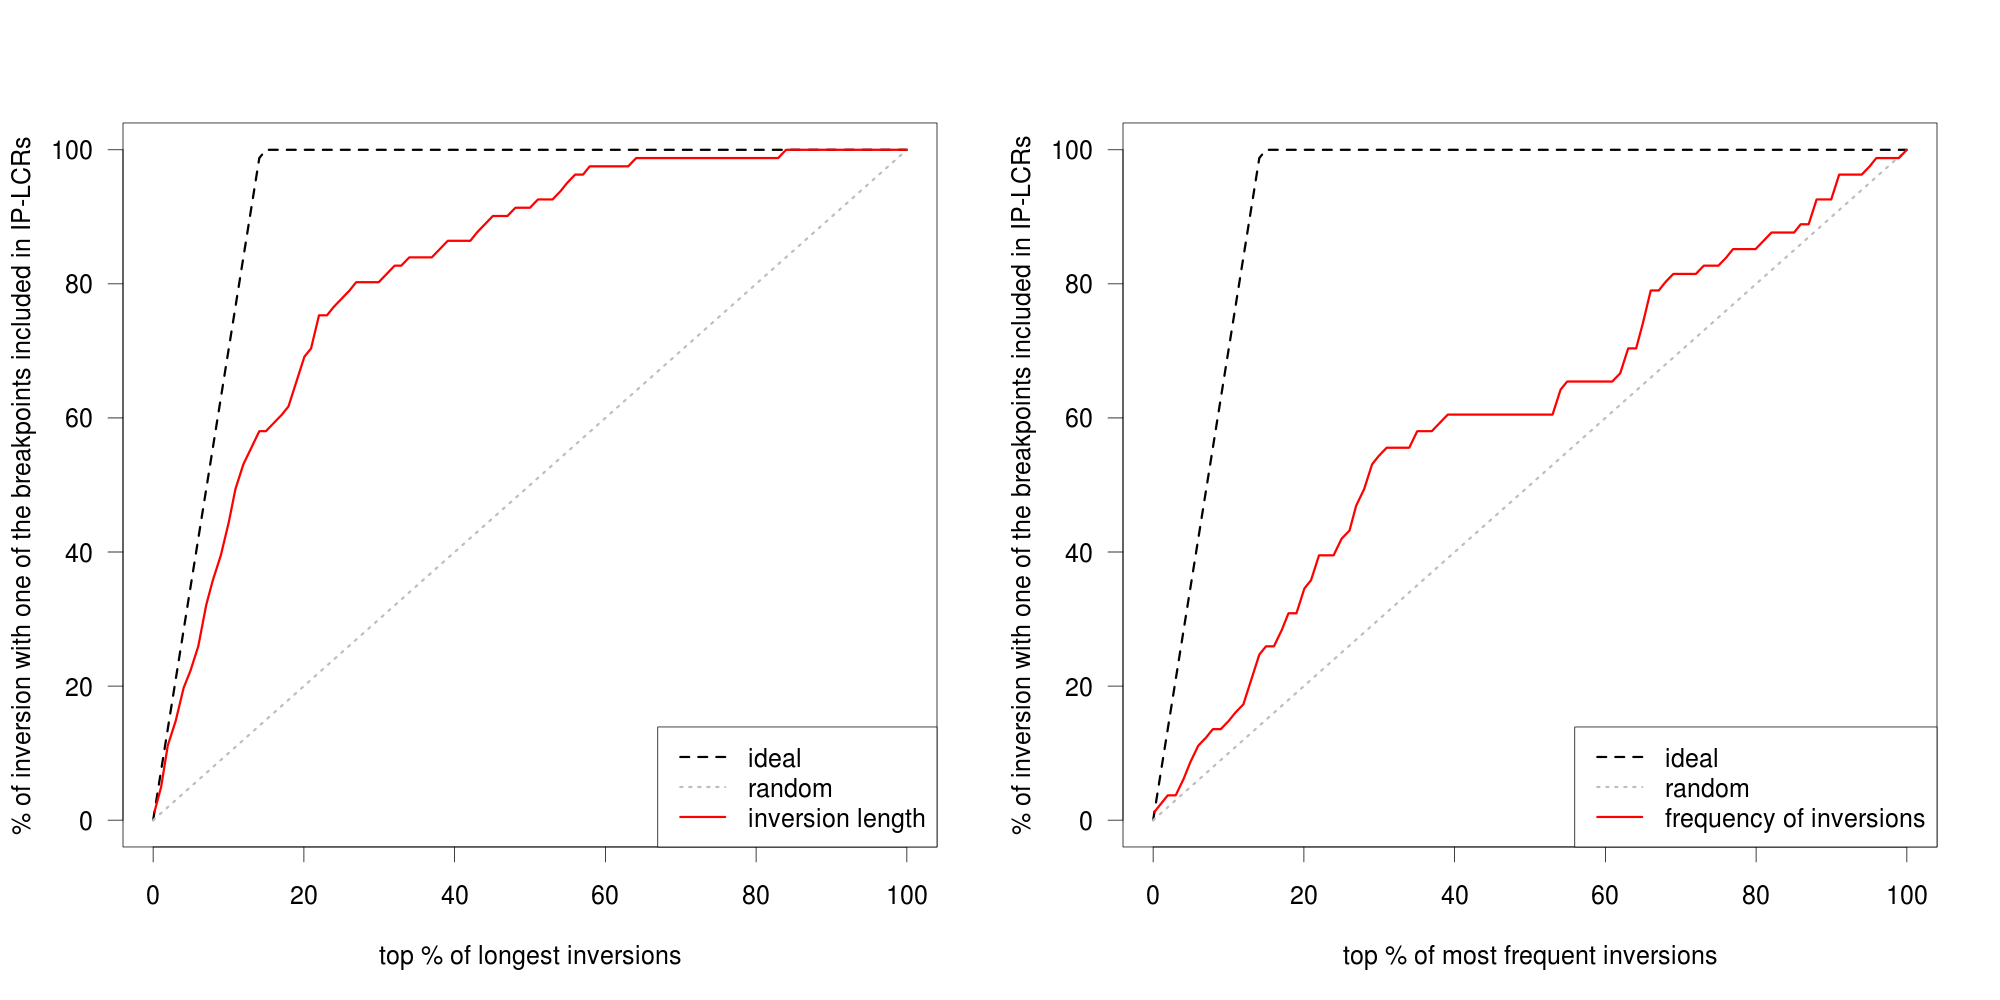
\includegraphics[width=1.1 \textwidth]{new-images/enrichments.png}\\
           \small{Enrichment curves for inversion size (left) and frequency of inversion occurence in
DGV (right) with respect to all inversions ($>$ 10 kb) with one or both breakpoints located inside
IP-LCR}
% 	   \tiny{source: Stankiewicz et al., 2002}  
% 	    \end{center}
\end{frame}





\begin{frame}\frametitle{Pathogenic inversions, DGV and IP-LCRs}  
% 	    \begin{center}
	   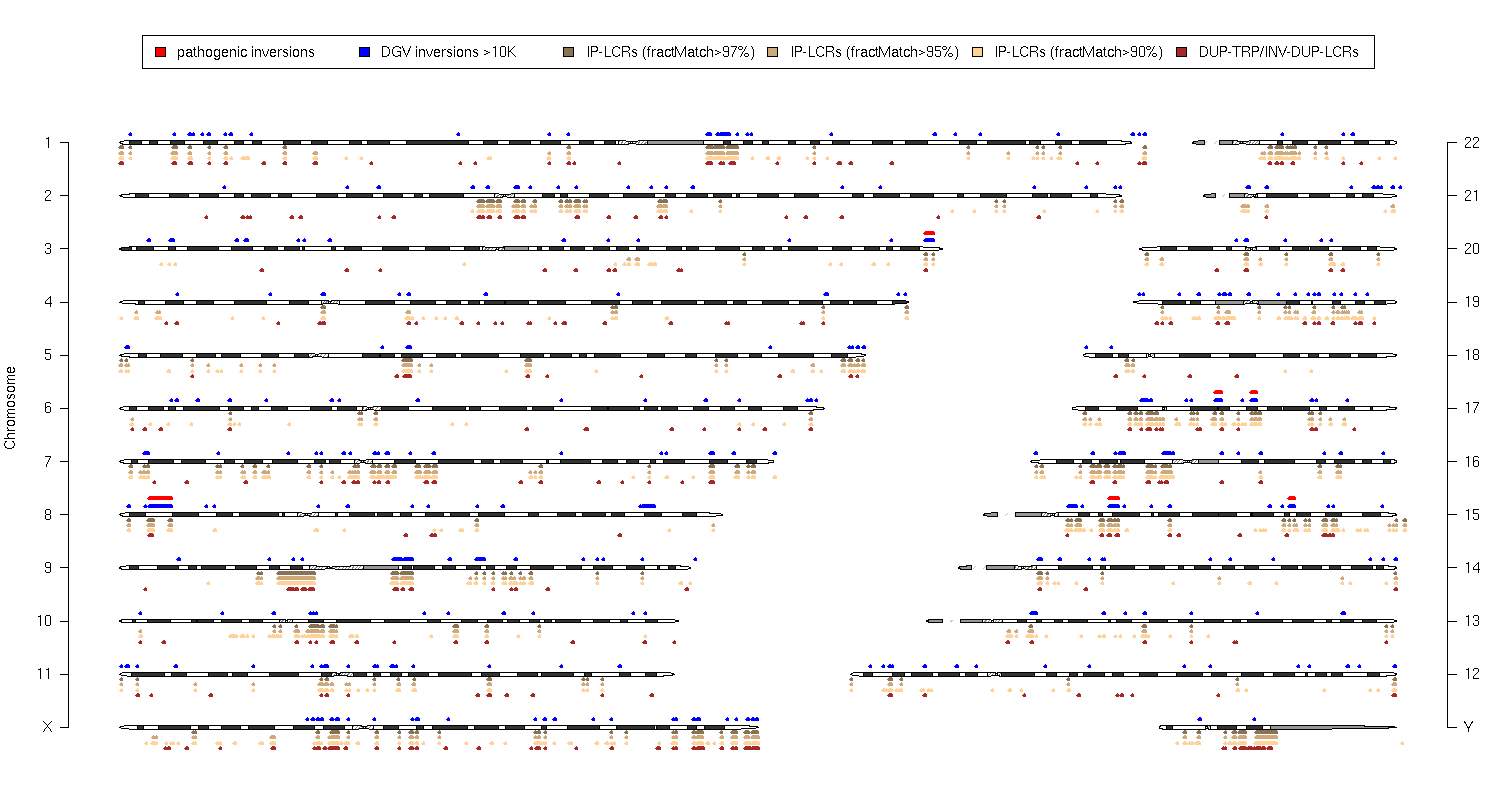
\includegraphics[width=1.1 \textwidth]{new-images/ideogram_inv_lcrs_new.png}\\
% 	   \tiny{source: Stankiewicz et al., 2002}  
% 	    \end{center}
\end{frame}



\begin{frame}\frametitle{Genomic Regions Enrichment of Annotations Tool (GREAT)}  
\begin{itemize} 
 \item input: set of genomic regions
 \item output: annotation terms significantly associated with inputs
 \item two kinds of tests for enrichment: binomial and hypergeometric
\end{itemize}
\end{frame}


\begin{frame}\frametitle{GREAT - selected results}  
 	   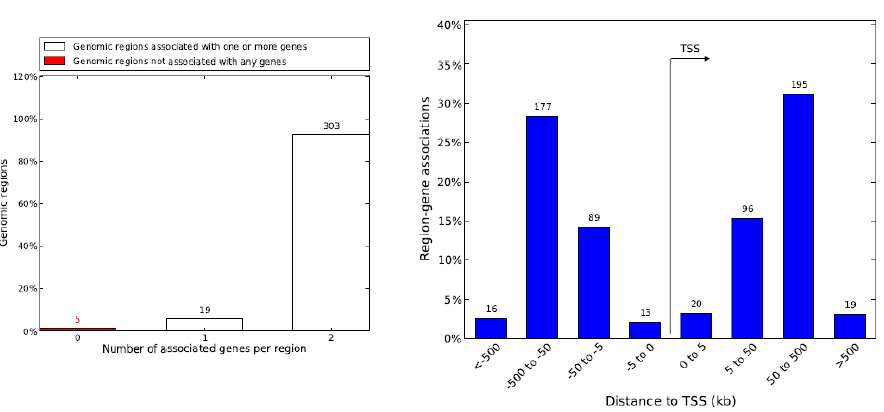
\includegraphics[width=\textwidth]{new-images/great.png}\\
\tiny{Number of associated genes per IP-LCR (left) and oriented distance to TSS (right) using GREAT version 1.8.2}
\end{frame}




\begin{frame}\frametitle{Binomial test (from GREAT)}  
\begin{itemize} 
 \item G - the size of the genome in base pairs.
 \item $g_{\pi}$ - the portion of the genome in the regulatory domain of a gene with annotation $\pi$. 
 \item $p_{\pi}$ = $g_{\pi}$ / G  
 \item n - the number of test genomic regions.
 \item $k_{\pi}$ - the number of test genomic regions in the regulatory domain of a gene with annotation $\pi$. 

\end{itemize}
The binomial p-value equals the probability of having $k_{\pi}$ or more of the n test genomic regions in the regulatory domain of a gene with annotation $\pi$ given that the probability of that occurring for a single genomic region is $p_{\pi}$.

$$\text{binomial p-value} = \sum_{i=k_\pi}^{n} {n\choose i}p_\pi^i(1-p_\pi)^{n-i}$$
% 	   \includegraphics[width=0.7\textwidth]{new-images/Binomial.png}\\

\end{frame}


% \begin{frame}\frametitle{Hypergeometric test}  
% \begin{itemize} 
%  \item 
%  \item 
%  \item 
% \end{itemize}
% \end{frame}

\begin{frame}\frametitle{Binomial test (our case)}  
\begin{itemize}  
 \item $g_{\pi}$ - the portion of the genome in the regulatory domain of a gene with annotation $\pi$. 
 \item $p_{\text{\tiny LCR}}$ - the proportion of human genome covered by IP-LCR regions
 \item $n$ - total number of inversions.
 \item $k$ - nr of inversions that intersect with at least one IP-LCR region

\end{itemize}
To  rectify the influence of (sometimes overestimated) inversion length we regard the inversion and IP-LCR region as intersecting if and only if the middle point 
of the inversion is located within the IP-LCR region.

$$
 \text{P-val}(k) = \sum_{i=k}^n {n \choose i} p_{\text{\tiny LCR}}^i (1-p_{\text{\tiny LCR}})^{n-i}
$$

\end{frame}


\begin{frame}\frametitle{Binomial test - results} 
The binomial test is often criticized as biased by a large number of genomic regions being associated with a small set of annotations (inversions in our case).
To minimize this  bias we  restrict our analysis to non-overlapping  inversions. 
\begin{table}[t!]
\begin{center}
\label{tab:binomial}
\begin{tabular}{c|c|c|c|c}
inversions  & $p_{\text{\tiny LCR}}$ & $n$ & $k$ & P-value \\\hline
all & 0.048 & 587 & 151 &  $<1E-64$\\\hline %$4.259514e-40$
non-overlapping & 0.048 & 334 & 73 & $<1E-26$\\%1.416723e-15.
\end{tabular}
\end{center}
\end{table}
\end{frame}



\begin{frame}\frametitle{DUP-TRP/INV-DUP LCRs}  
\begin{itemize} 
 \item 100\% identical repeated sequences of inverted orientation and minimum length of 145 bp,
 \item inverted repeated sequences used as seeds to extend and merged into larger regions or tracks of $>$ 98\% identity,
 \item these repeated tracks were then filtered by size to those larger than 820 bp and separated by 30 kb and up to 350 kb,
consistent with previous experimental observations (Carvalho et al. 2011),
 \item repeated sequences were merged and analyzed using custom-made Perl scripts.
 \item finally 1385 LCRs obtained 
\end{itemize}
\end{frame}


\begin{frame}\frametitle{Pathogenic inversions, DGV and LCRs}  
% 	    \begin{center}
	   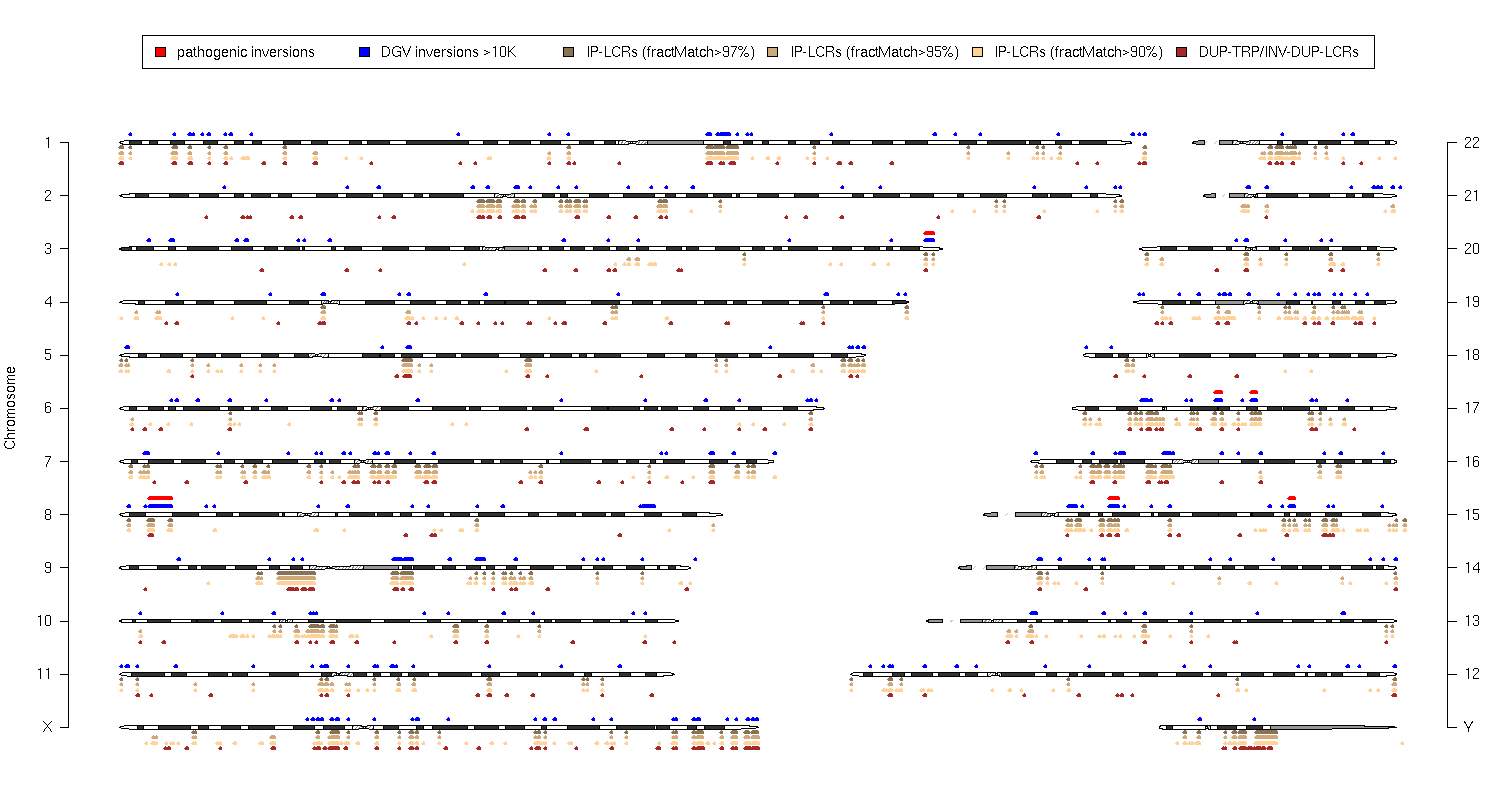
\includegraphics[width=1.1 \textwidth]{new-images/ideogram_inv_lcrs_new.png}\\
% 	   \tiny{source: Stankiewicz et al., 2002}  
% 	    \end{center}
\end{frame}






\begin{frame}\frametitle{Gene conversions}  
\begin{itemize} 
 \item 797 identified genes have been reported to be inactivated by gene conversion
events between the inverted LCR copies
 \item Among them, there are 24 genes considered as dosage sensitive by Huang et al.
(2010)
 \item 18 genes have been associated with different diseases or syndromes
\item To (automatically) assign the phenotypes to other genes, we have used the Genetic
Association Database (GAD) and the Mouse Genome Database (MGD) resources
\item the distribution among the different disease classes for genes potentially disrupted by the rearrangements mediated by the IP-LCRs does not reveal any
highly dominant disease class
\end{itemize}
\end{frame}


\begin{frame}\frametitle{Genetic Association Database (GAD)}  
\begin{itemize}  
 \item http://geneticassociationdb.nih.gov/
 \item goal: \textit{allow to rapidly identify medically relevant polymorphism from the large volume of polymorphism and mutational data, in the context of standardized nomenclature} 
\end{itemize}
\begin{center}
	   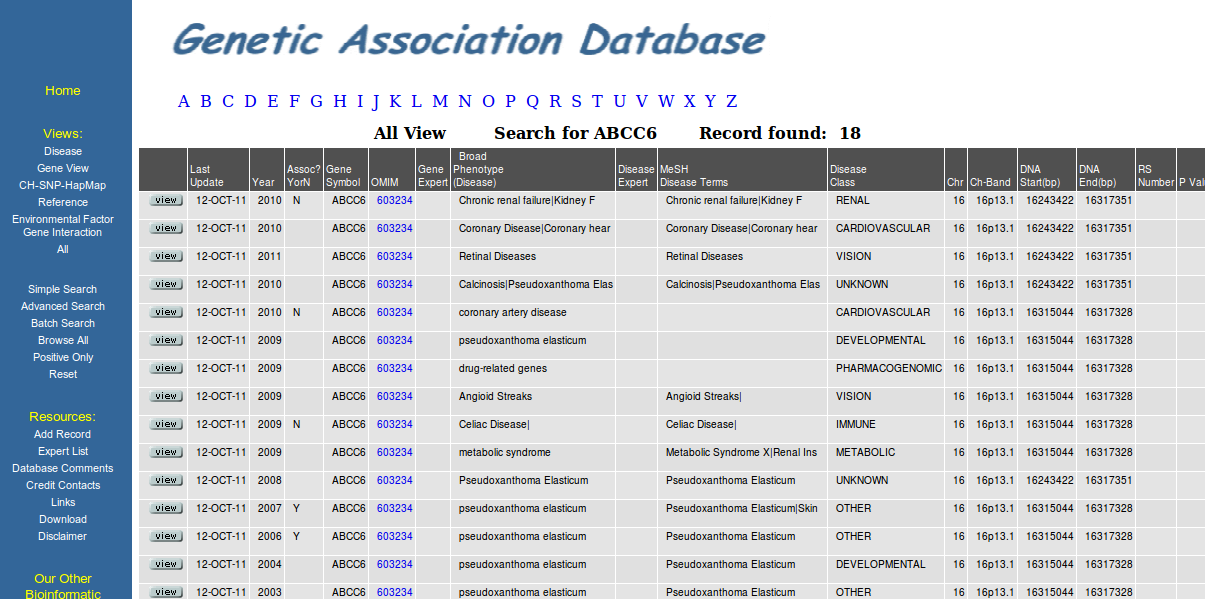
\includegraphics[width=0.9 \textwidth]{new-images/GAD.png}\\	   
	    \end{center}
\end{frame}


\begin{frame}\frametitle{Mouse Genome Database (MGD)}  

\begin{center}
	   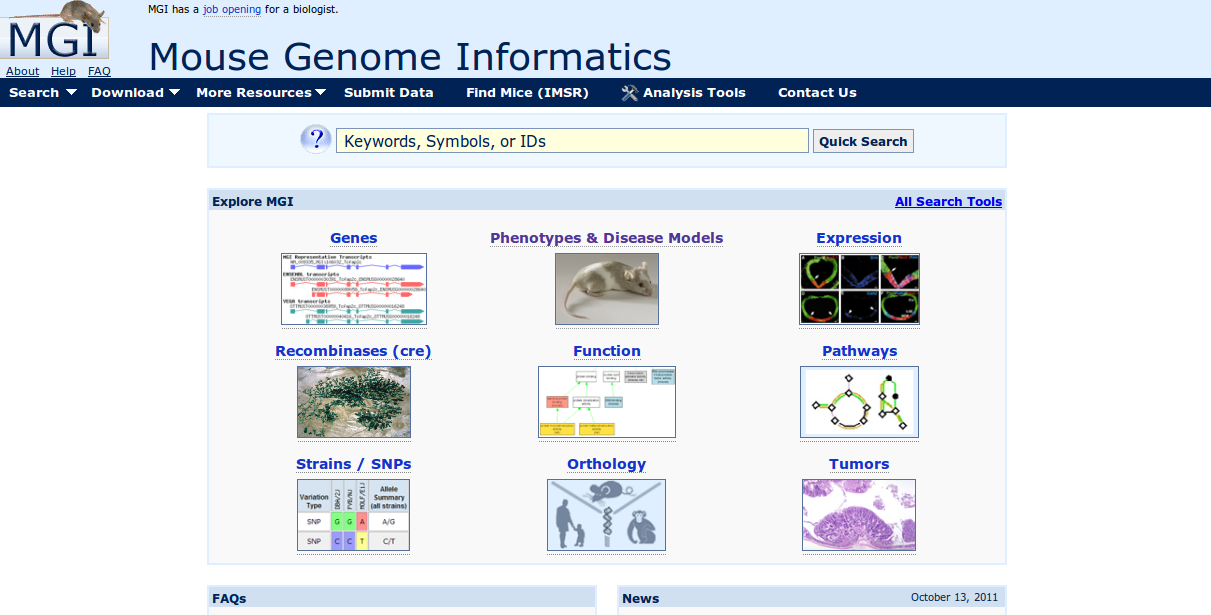
\includegraphics[width=0.9 \textwidth]{new-images/MGD.png}\\	   
	    \end{center}

\begin{itemize}  
 \item http://www.informatics.jax.org/
 \item \textit{data on gene characterization, nomenclature, mapping, gene homologies among mammals, sequence links, phenotypes, allelic variants and mutants, and strain data} 
\end{itemize}

\end{frame}





\begin{frame}\frametitle{Genes - cont.}  
\begin{figure}
 \centering  
 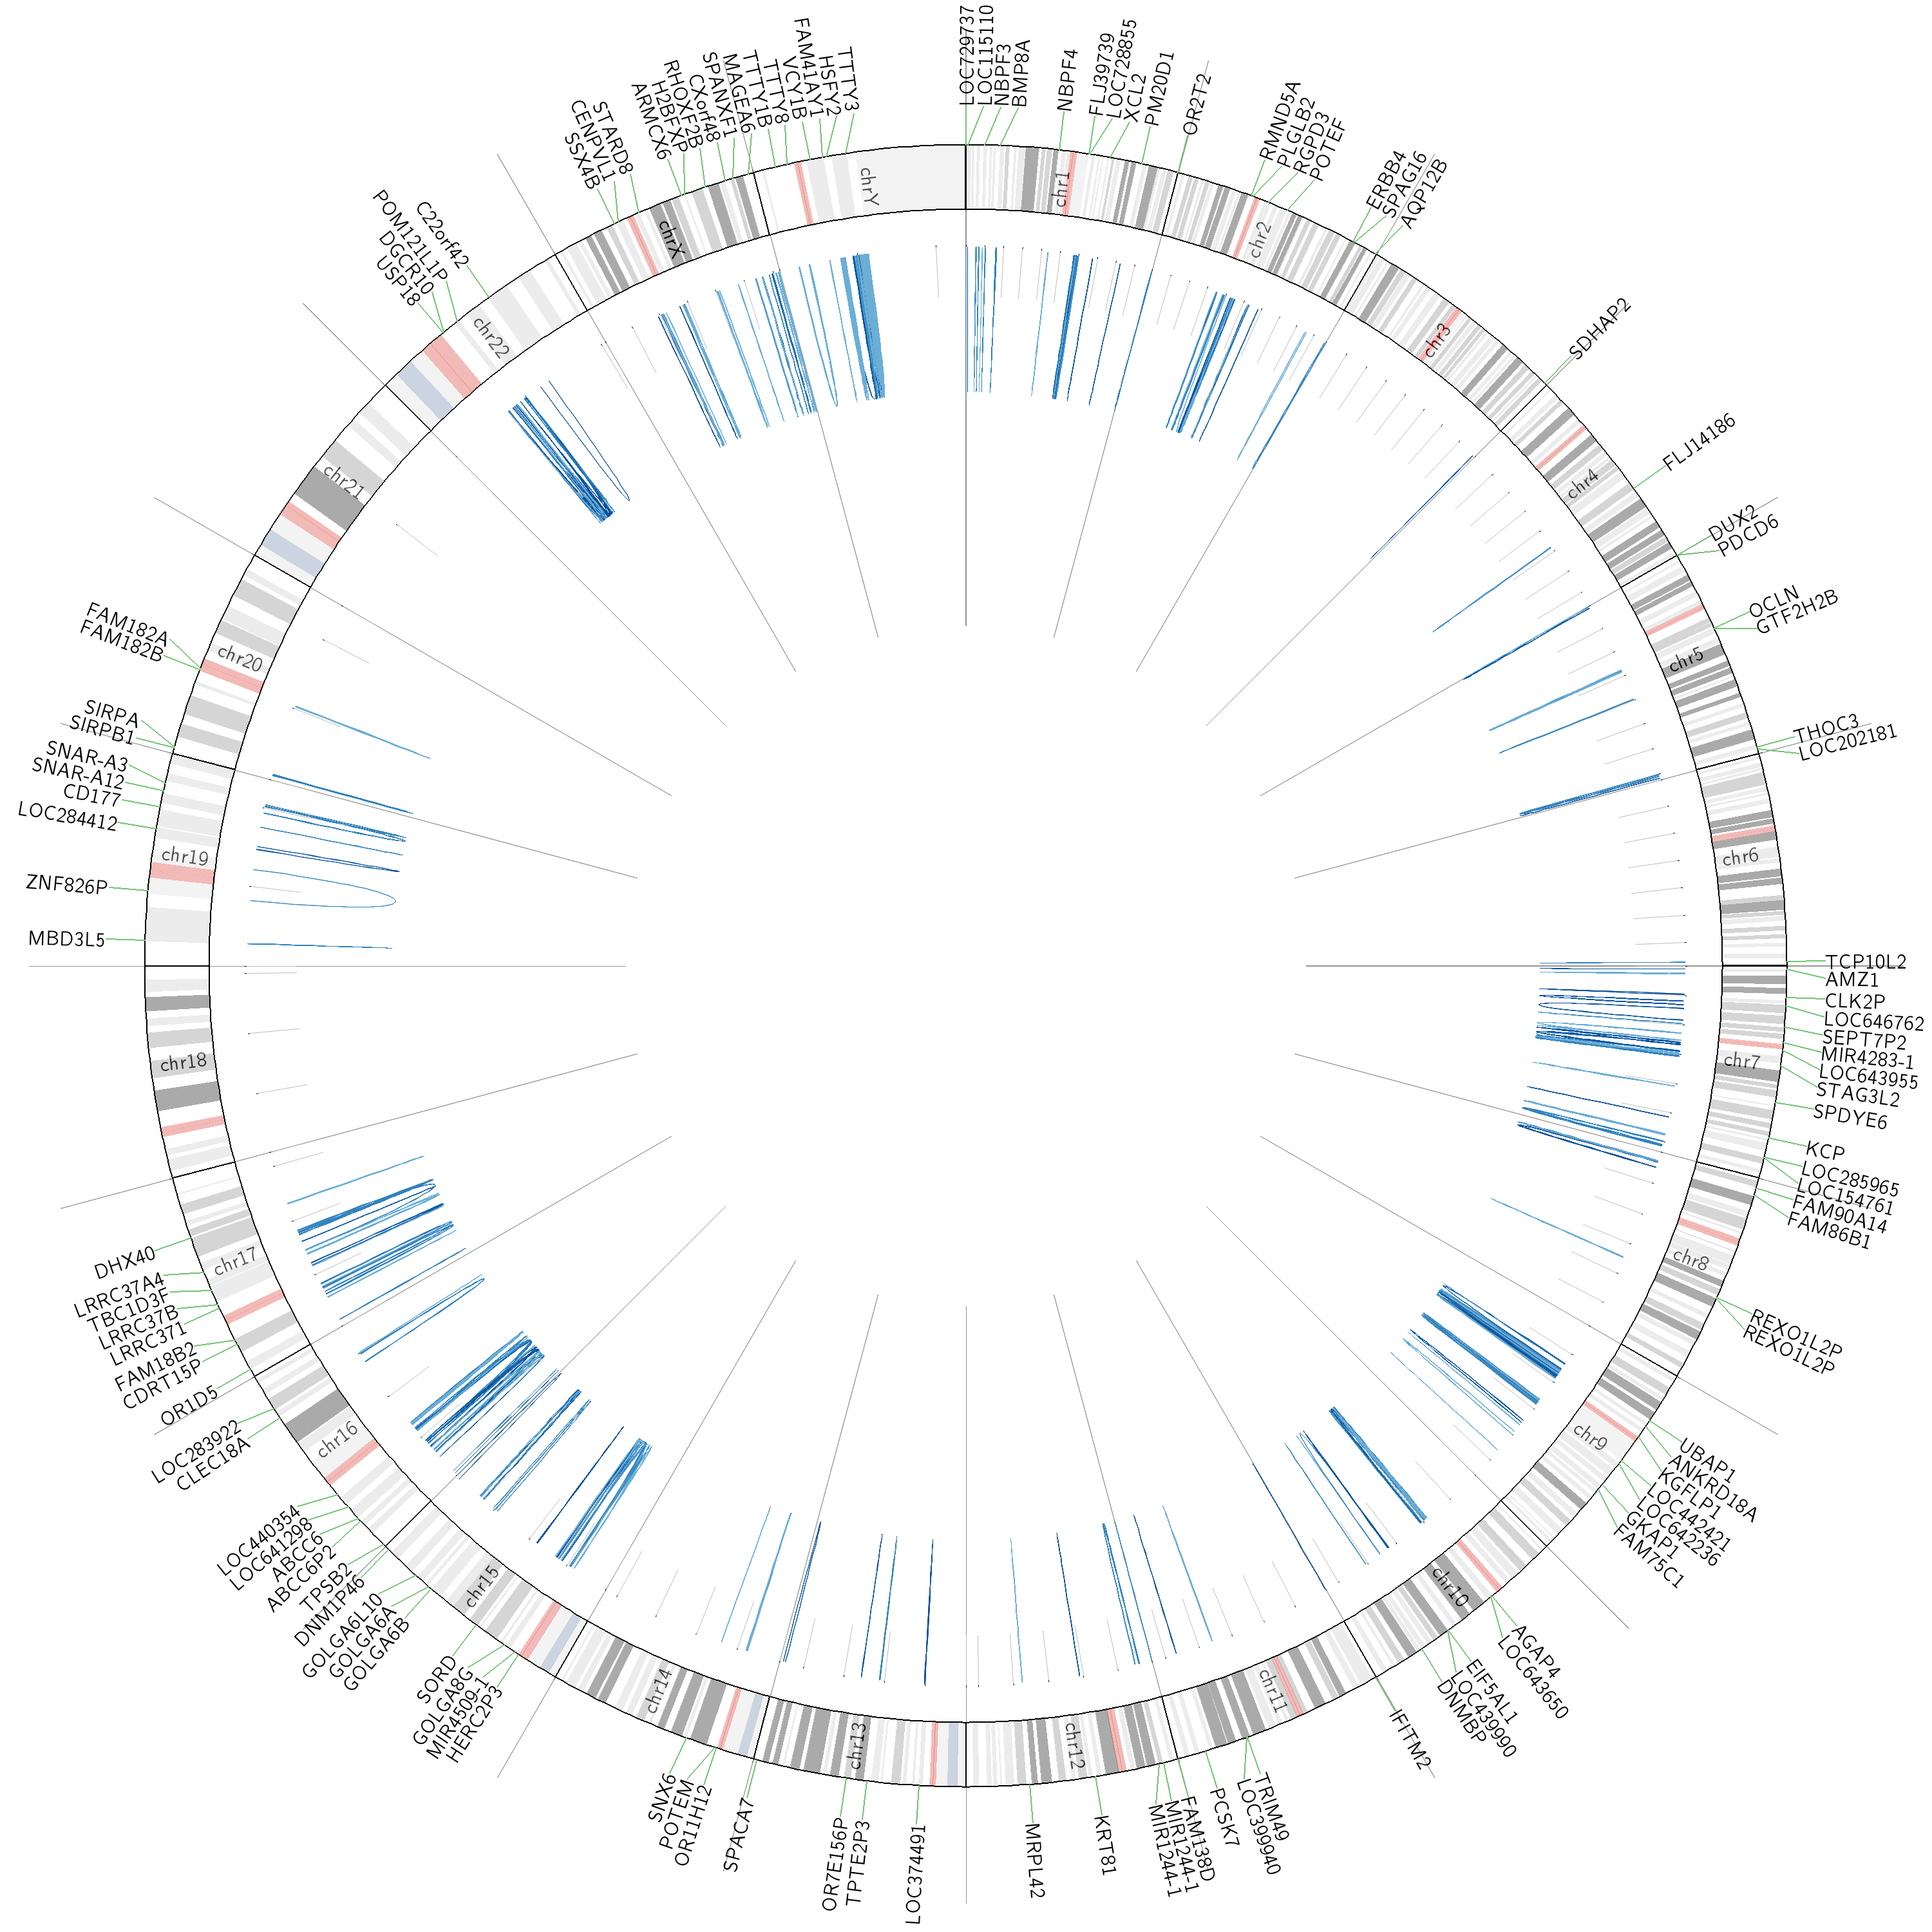
\includegraphics[width=.45 \textwidth]{new-images/all_chromosomes.png}
 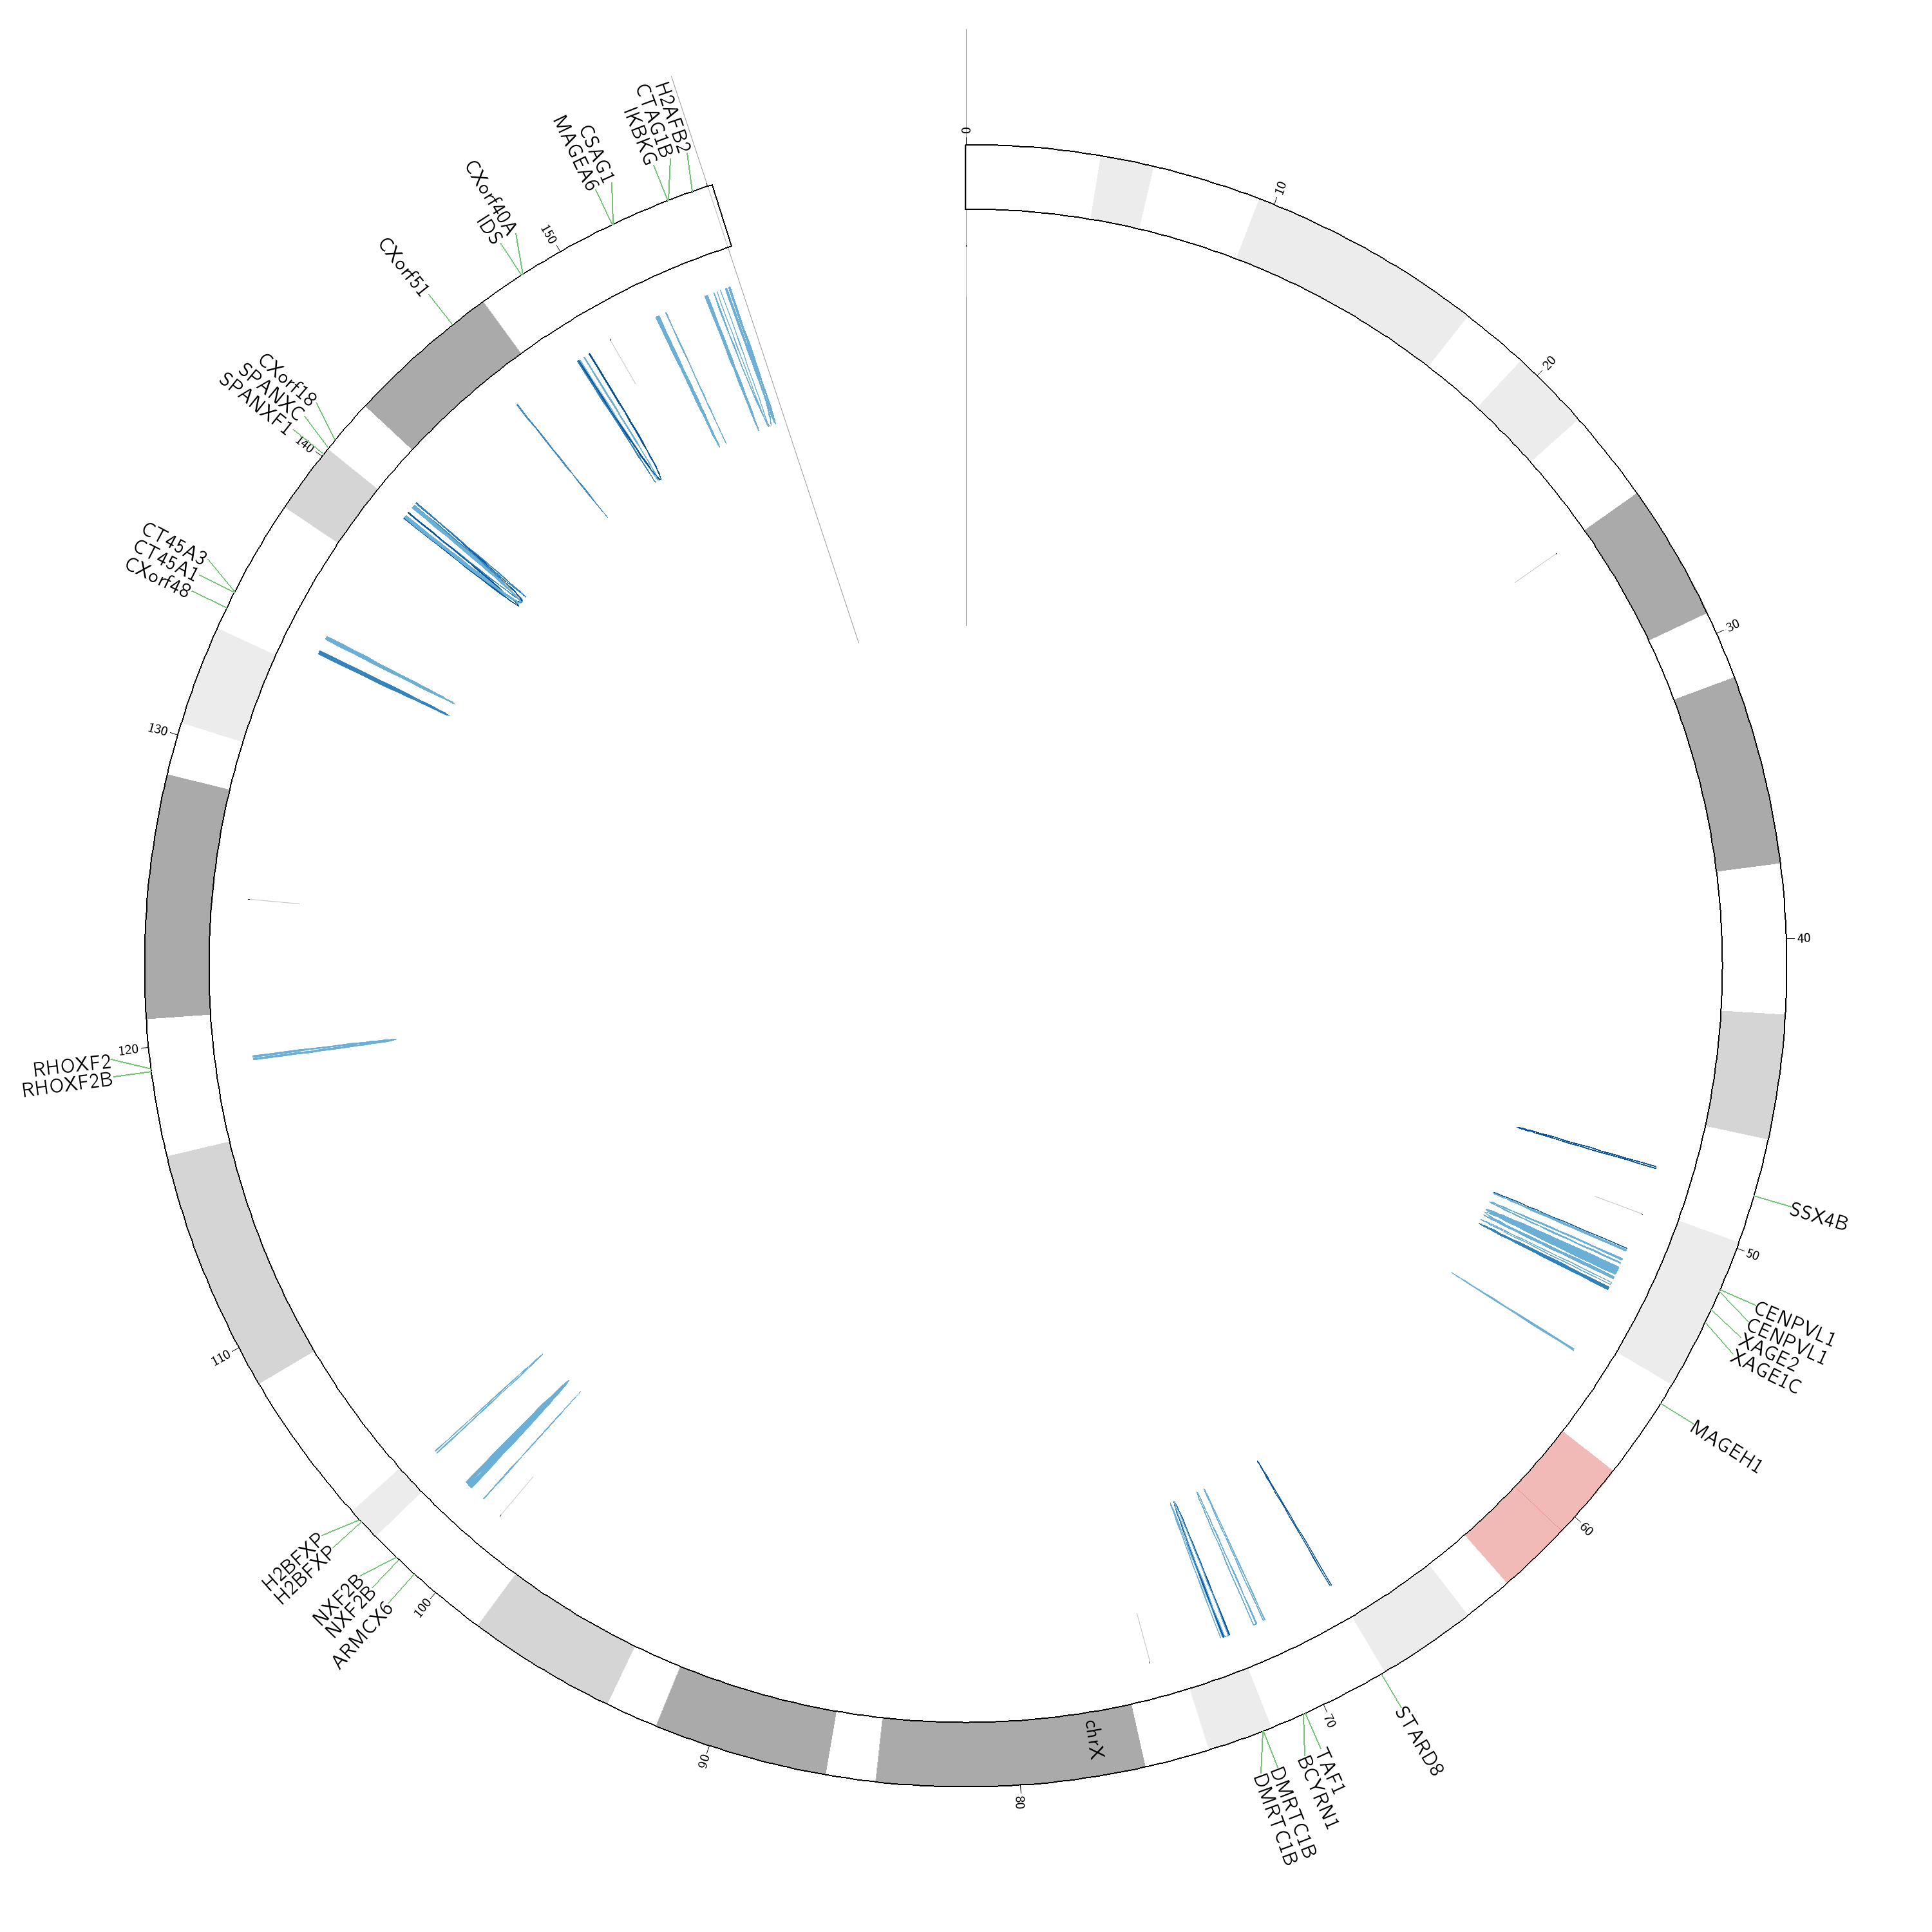
\includegraphics[width=.45 \textwidth]{new-images/chrX.png} 
 \label{fig:nitrogen_lipids}
\caption{(left) IP-LCRs (fraction matching above .97) on the whole human genome and
(right) on chromosome X. Light-dark color scale shows the ascending fraction matching between IP-LCRs.}
\end{figure}
\end{frame}

\begin{frame}\frametitle{Fraction matching vs. IP-LCRs}  
% 	    \begin{center}
	   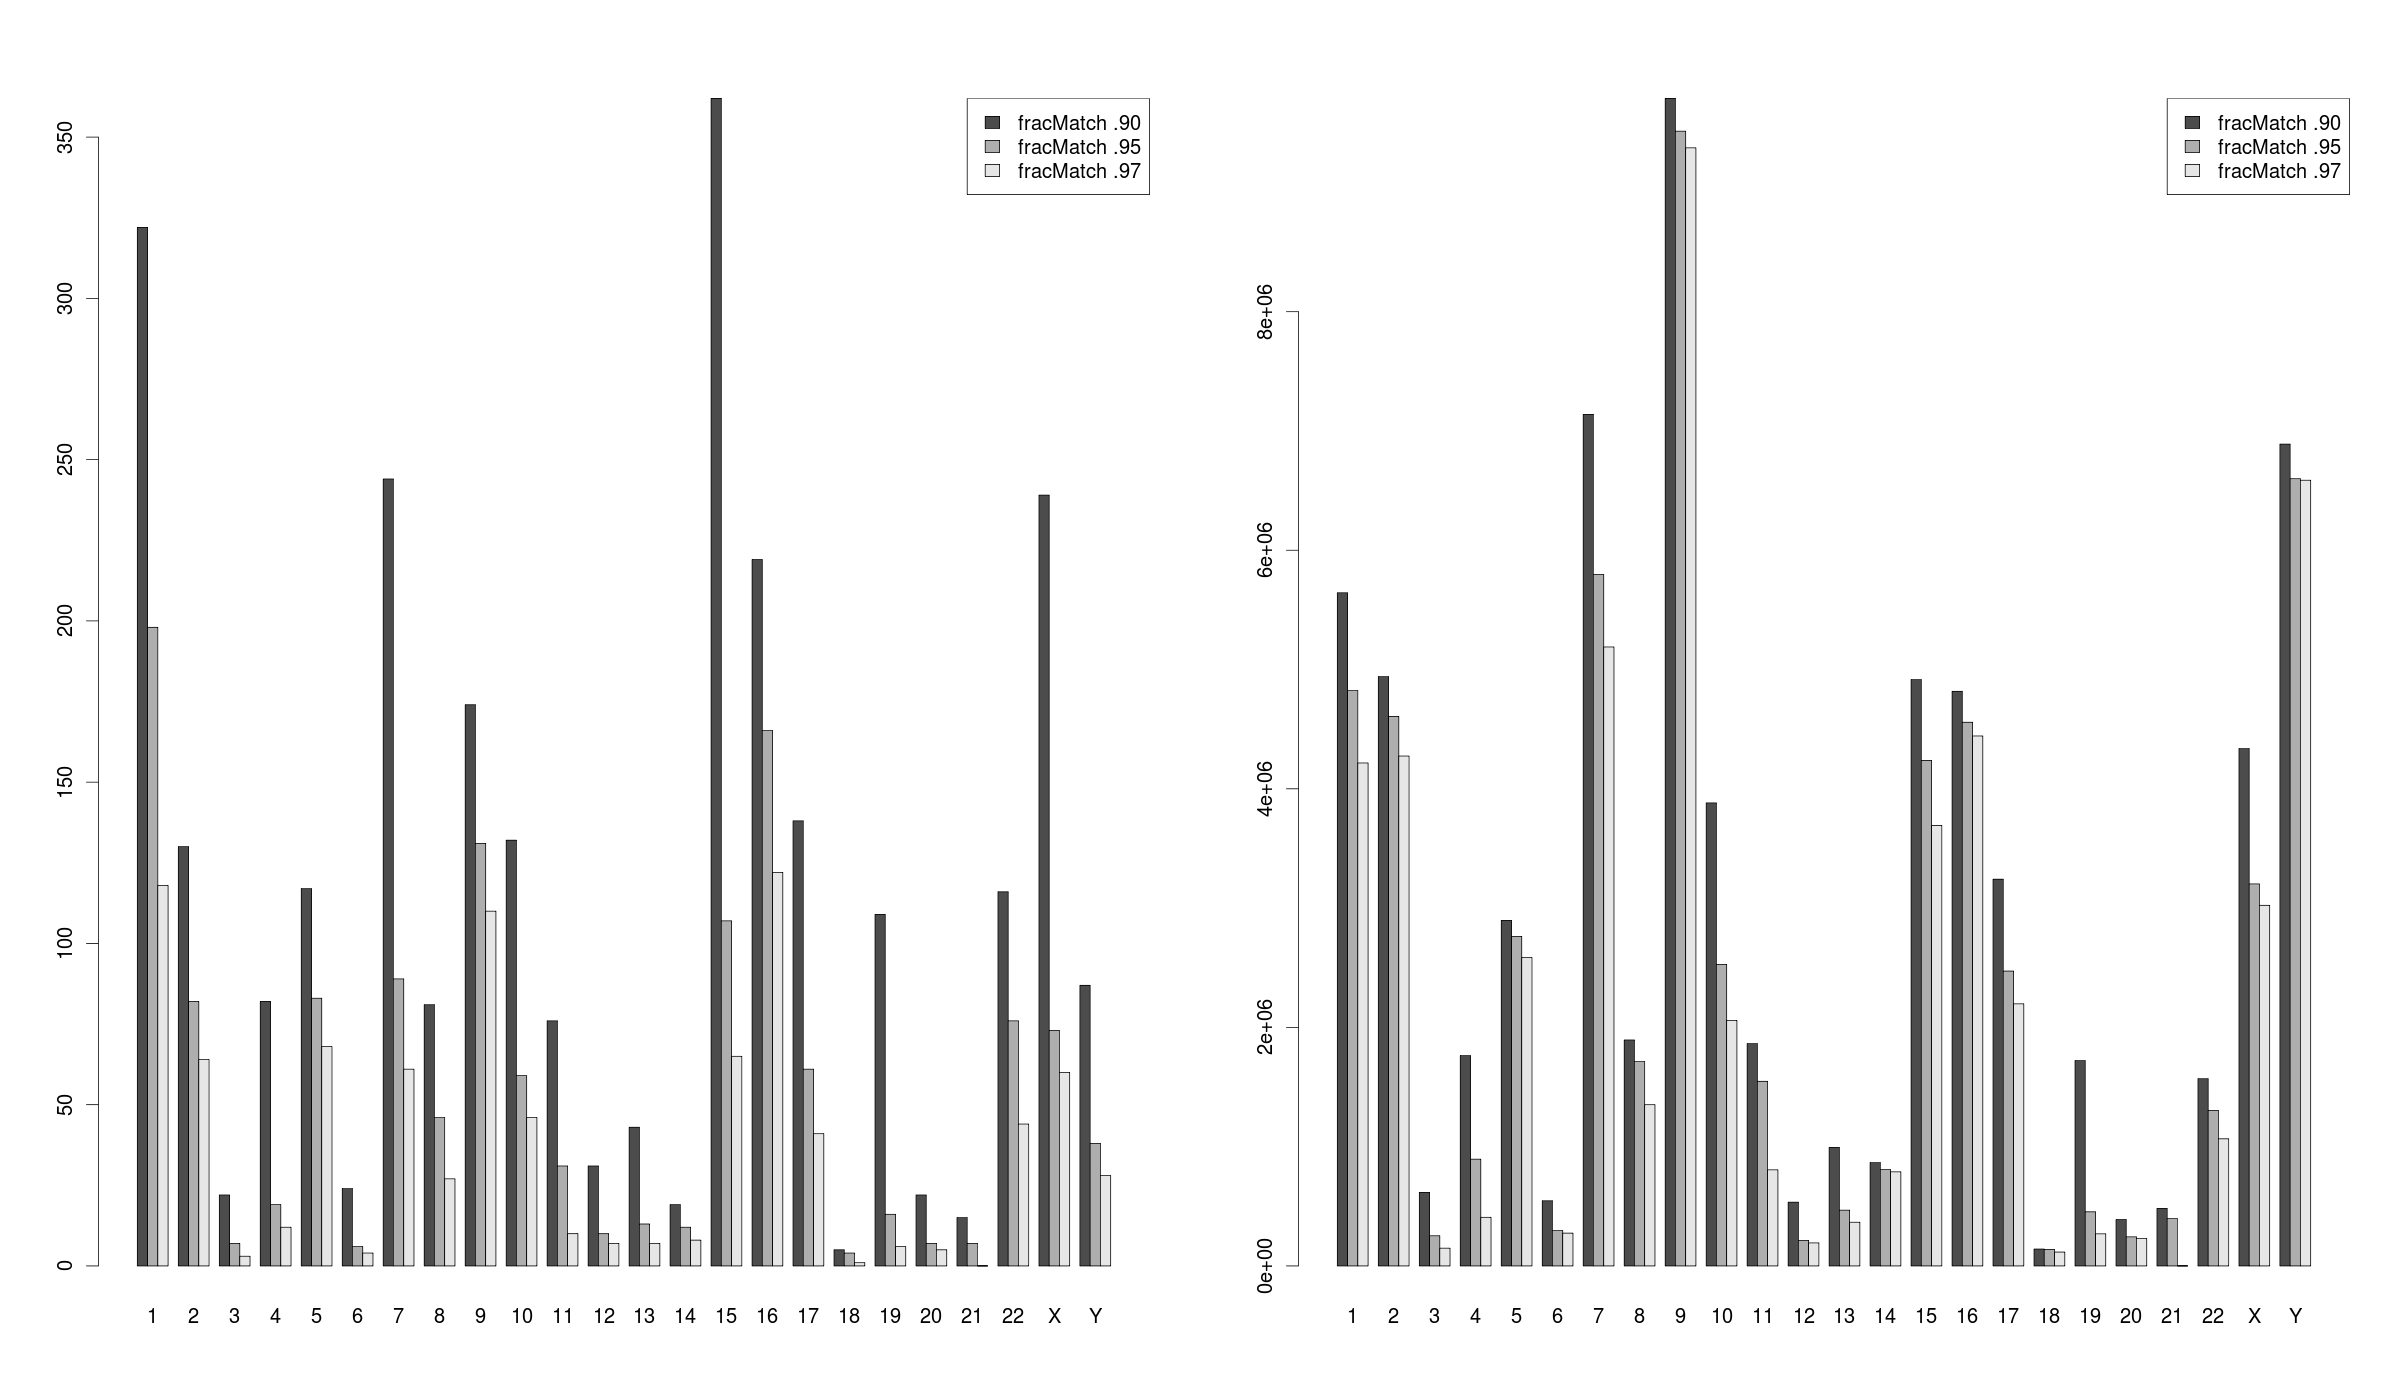
\includegraphics[width= \textwidth]{new-images/hist_lcrs_distances_chrom.png}\\
Distribution of number of IP-LCRs (left) and base pair length of IP-LCRs (right) on all 24 chromosomes.
% 	   \tiny{source: Stankiewicz et al., 2002}  
% 	    \end{center}
\end{frame}

\begin{frame}\frametitle{Genes vs. DTIP-LCRs} 
\begin{itemize}
 \item 5,338 genes located upstream, downstream, or in between of a pair of inverted tracks and up
to 1 Mb upstream or downstream, based on experimental observations of DUP-TRP/INV-DUP rearrangements. 
 \item  1,394 disease associated genes that are are at risk of undergoing copy-number gain as a consequence of formation of a DUP-TRP/INV-DUP kind of rearrangement 
\end{itemize}
% \begin{figure}
%  \centering  
%  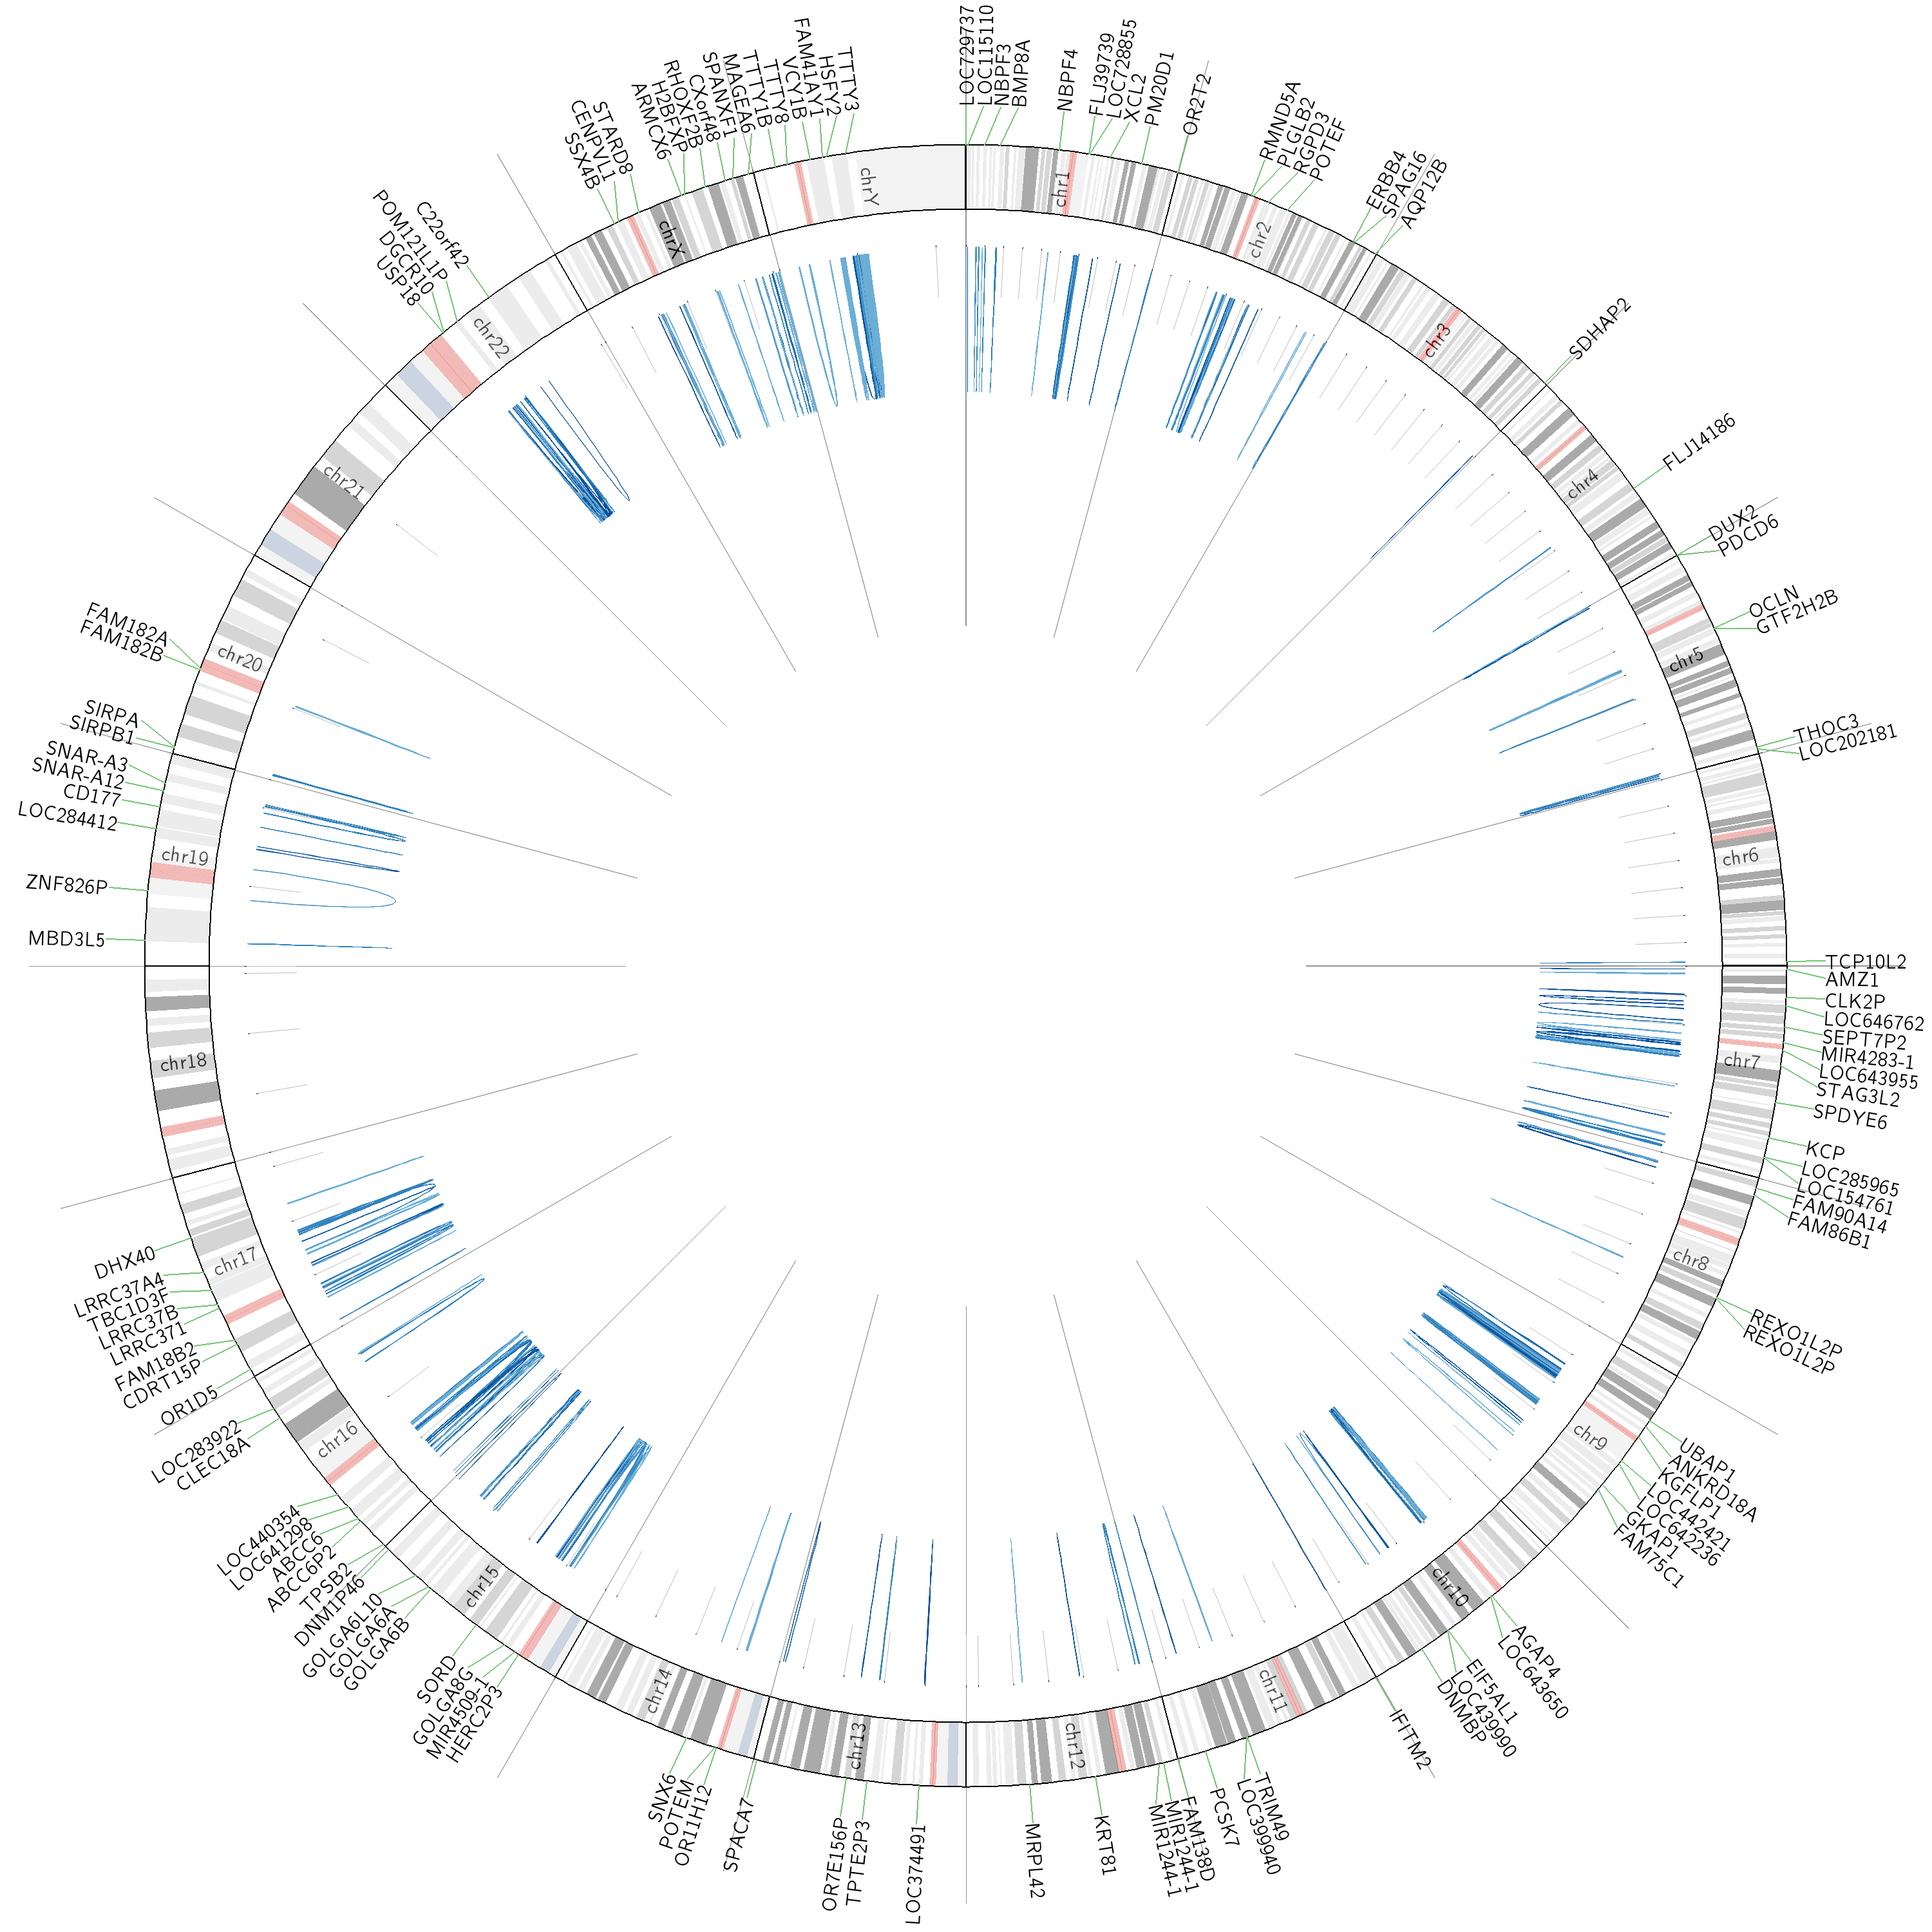
\includegraphics[width=.45 \textwidth]{new-images/all_chromosomes.png}
%  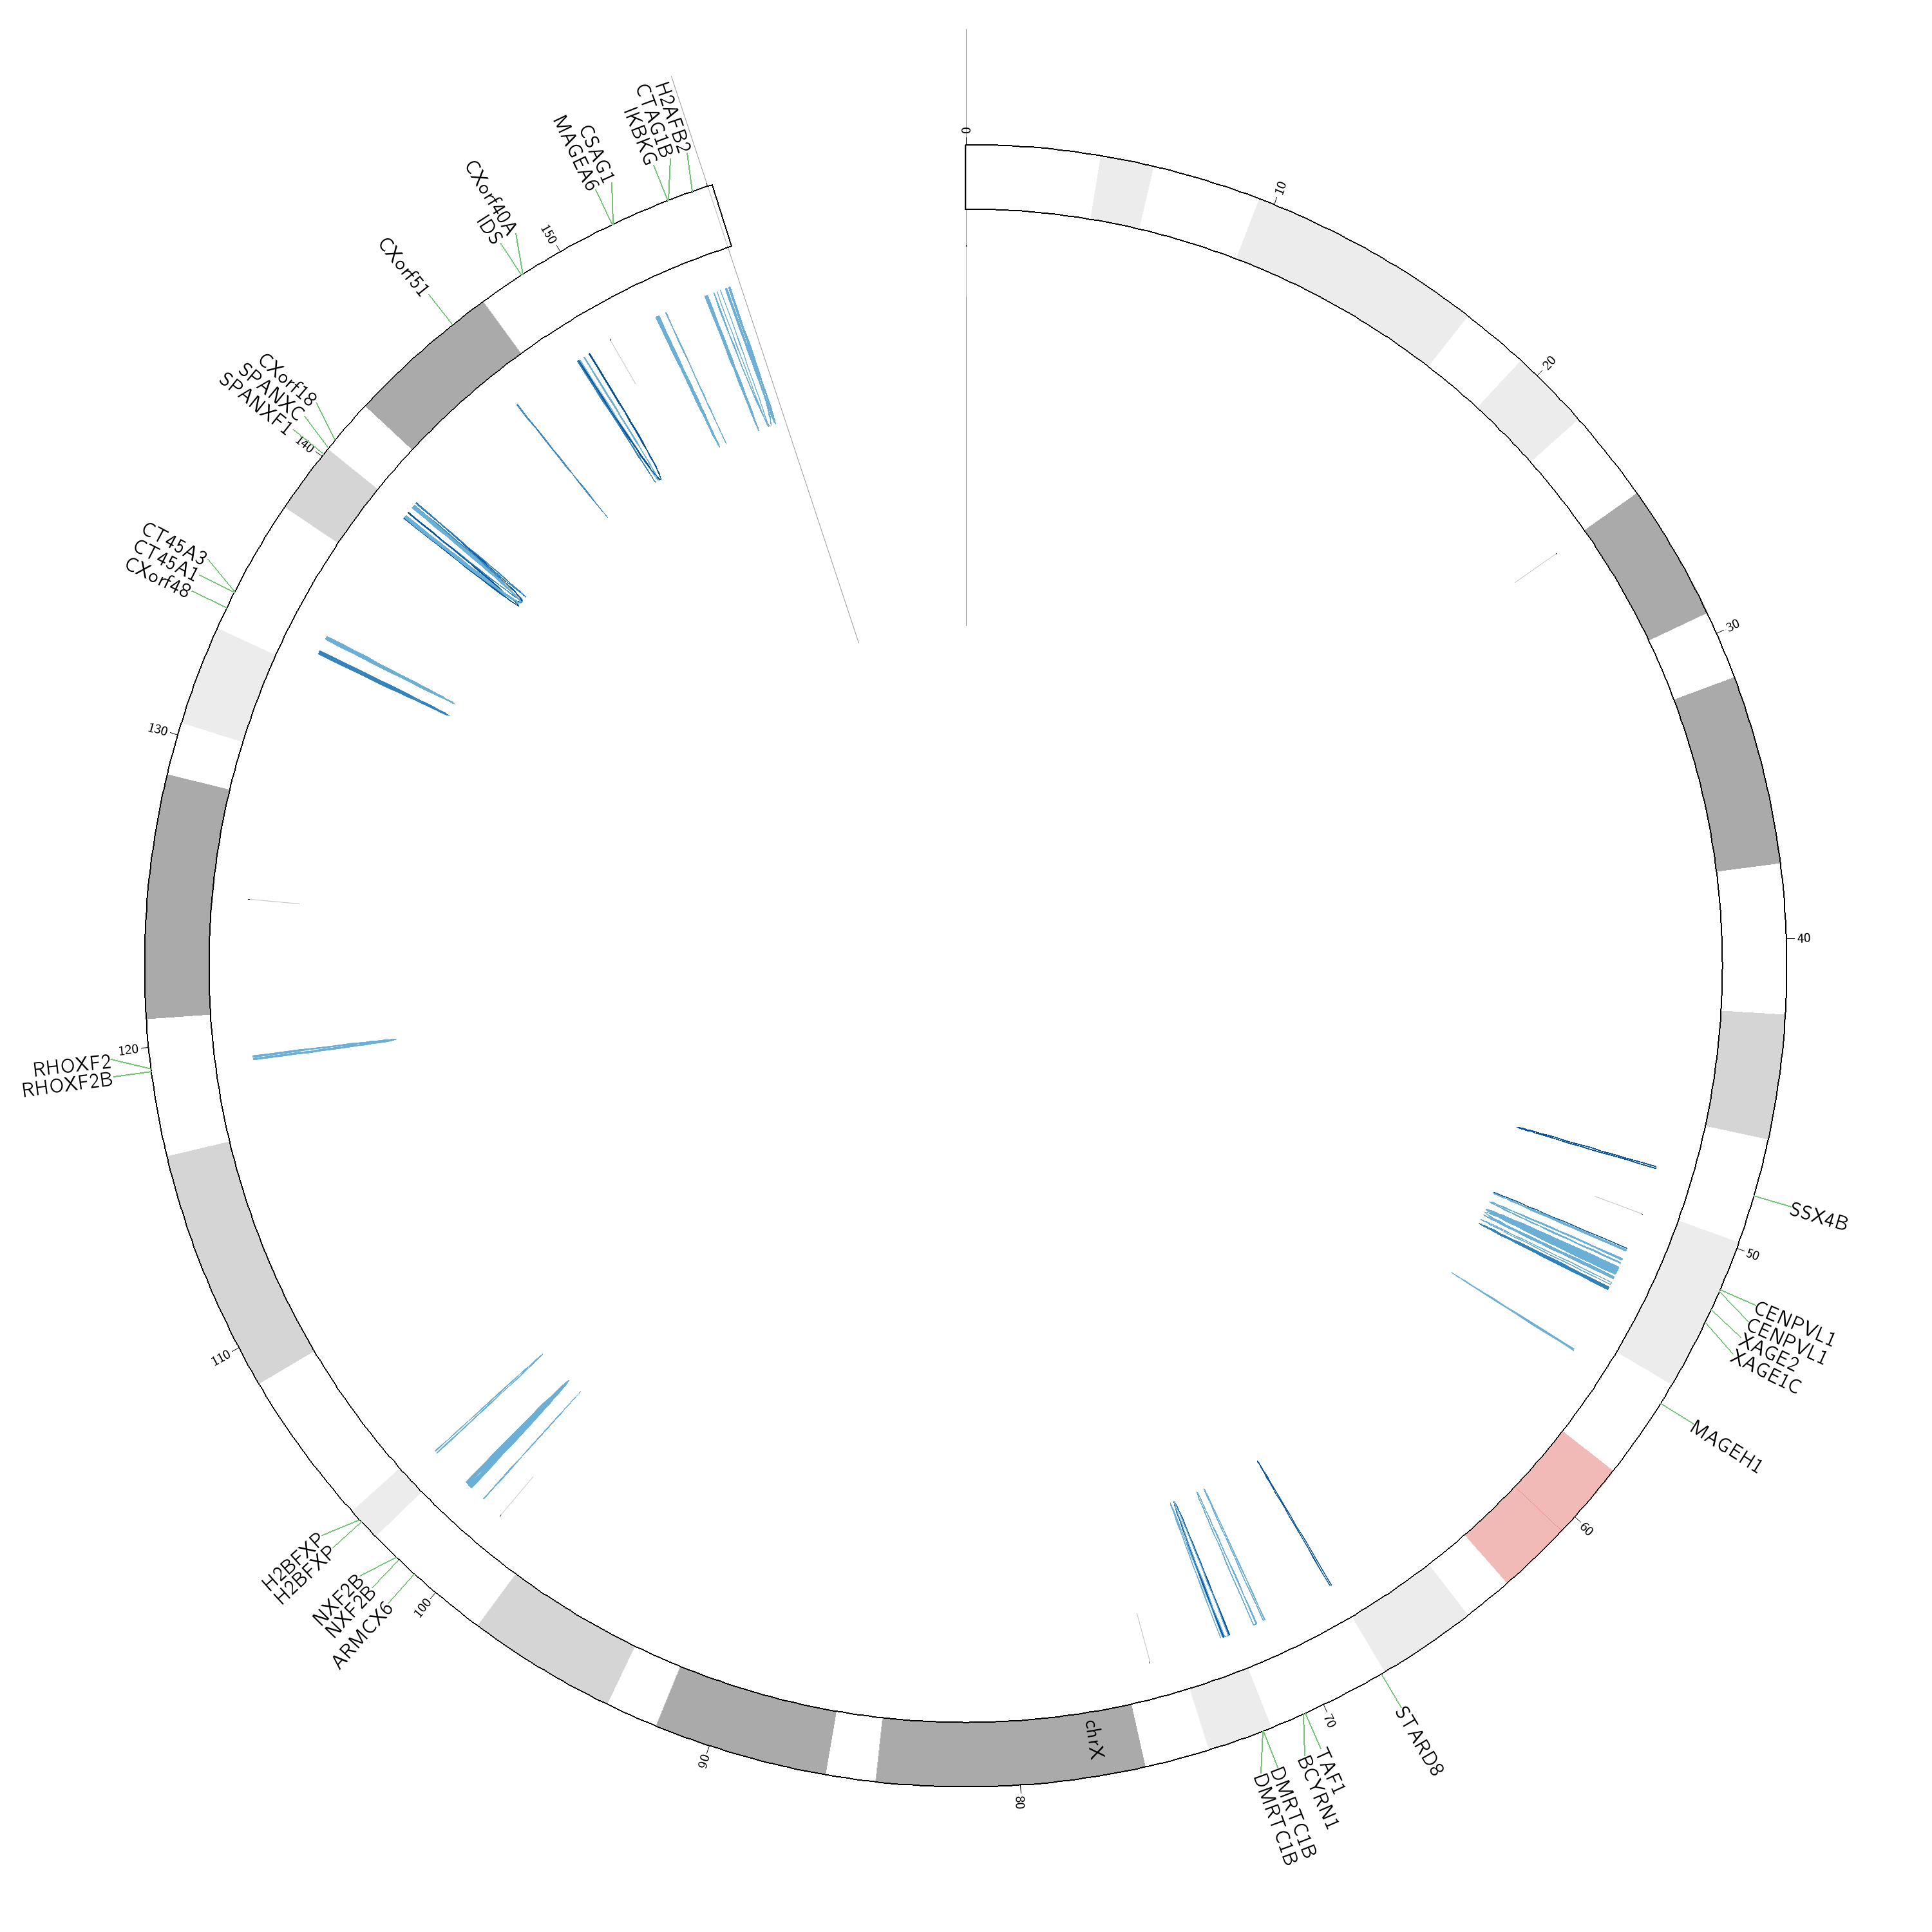
\includegraphics[width=.45 \textwidth]{new-images/chrX.png} 
%  \label{fig:nitrogen_lipids}
% \caption{(left) IP-LCRs (fraction matching above .97) on the whole human genome and
% (right) on chromosome X. Light-dark color scale shows the ascending fraction matching between IPLCRs.}
% \end{figure}
\end{frame}


\begin{frame}\frametitle{DUP-TRP/INV-DUP mechanism}  
% 	    \begin{center}
	   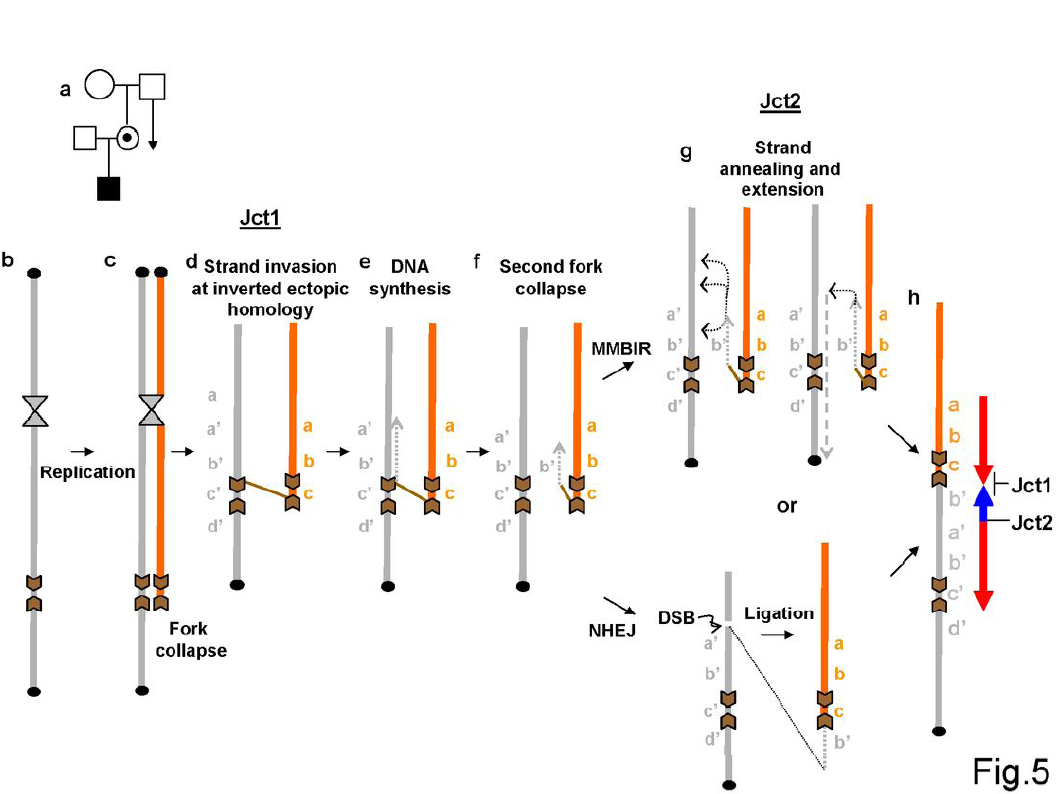
\includegraphics[width=1 \textwidth]{new-images/DTIP.png}\\
\end{frame}

\begin{frame}\frametitle{DUP-TRP/INV-DUP mechanism - identification}  
% 	    \begin{center}
	   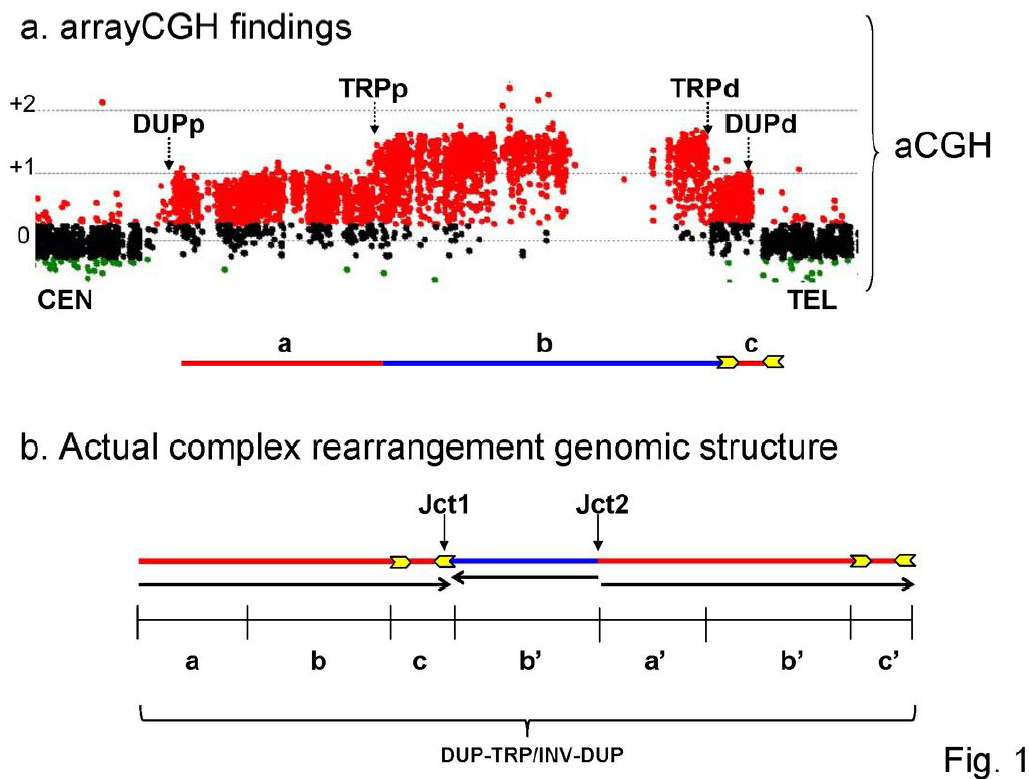
\includegraphics[width=1 \textwidth]{new-images/aCGH-DTIP.png}\\
\end{frame}




\begin{frame}\frametitle{Further steps} 
\begin{itemize}
 \item detailed analysis of the correlation between LCRs characteristics and recurrent inversions
 \item flexible parametrization of UCSC track (e.g. for relaxing the minimal length restriction)
\end{itemize}
\end{frame}
 


